\begin{exercice}
Antoine possédait 832,25 CHF sur son livret d'épargne. Pour son anniversaire, ses parents y ont déposé 75 CHF. Combien a-t-il maintenant sur son livret ?
\end{exercice}


\begin{exercice}
Un panier plein de fruits pèse 1,836 kg. Vide, il pesait 0,425 kg. Quelle est la masse des fruits contenus dans ce panier ?
\end{exercice}


\begin{exercice}
Pierre a relevé le compteur de sa voiture au départ et au retour de vacances. Au départ, le compteur indiquait 58\,257,6 km. Au retour, il indiquait 59\,329,1 km. Quelle distance a‑t‑il parcourue pendant ses vacances ?
\end{exercice}


\begin{exercice}
Simon veut acheter un livre. Il a 25,35 CHF dans son porte‑monnaie et il lui manque 5,25 CHF pour acheter ce livre. Quel est le prix du livre ?
\end{exercice}


\begin{exercice}
Une voiture consomme 8,5 l d'essence pour faire 100 km. Combien d'essence consomme‑t‑elle pour faire 500 km ?
\end{exercice}
  
  
\begin{exercice}
Un employé gagne 17,25 CHF de l'heure. Il travaille 35 heures par semaine. Combien gagne‑t‑il chaque semaine ?
\end{exercice}


\begin{exercice}
Au marché, Anne a déposé dans son panier 1,2 kg de carottes, 600 g de raisin et 1,3 kg de pommes. Combien pèse le contenu de son panier ?
\end{exercice}


\begin{exercice}
Pour aller au collège, Caroline fait 1,4 km avec son vélo qu'elle laisse chez sa grand‑mère. Puis elle parcourt 150 m à pied jusqu'au collège. Quelle distance totale parcourt‑elle pour se rendre au collège ?
\end{exercice}


\begin{exercice}
Djamel a acheté 1,6 kg de poires à 2,30 CHF le kg. Combien a‑t‑il payé ?
\end{exercice}


\begin{exercice}
Gérard a payé 41,40 CHF pour 12 pieds de tomate. Quel est le prix d'un pied de tomate ?
\end{exercice}



\begin{exercice}
Un lot de six stylos identiques coûte 8,10 CHF. Quel est le prix d'un stylo ?
\end{exercice}


\begin{exercice}
Mercredi après‑midi, Anh Hao a fait cinq tours d'un circuit de VTT. Il a parcouru en tout 23,5 km. Quelle est la longueur de ce circuit ?
\end{exercice}


\begin{exercice}
Mme Betty possède 6,6 litres de jus de pomme. Combien de bouteilles de 0,7 litres pourra-t-elle remplir ?
\end{exercice}

\begin{exercice}
Agan possède 37,40 CHF en pièces de 20 centimes. Combien de pièces de 20 centimes possède t'il ?
\end{exercice}


\begin{exercice}[Calculer sans poser]


\begin{enumerate}
 \item Calcule mentalement les produits suivants sachant que $6,5 \times 3,7 = 24,05$ :
 \begin{colitemize}{3}
  \item $6,5 \times 37$ ;
  \item $65 \times 37$ ;
  \item $6,5 \times 0,37$ ;
  \item $0,65 \times 3,7$ ;
  \item $6\,500 \times 0,003\,7$ ;
  \item $65 \times 0,37$.
  \end{colitemize}
  
 \item Sachant que $935 \div 17 = 55$, que dire des quotients suivants ? Justifie.   
 \begin{colitemize}{2}
  \item $9 350 \div 170$ ;
  \item $93,5 \div 1,7$ ;
  \item $93\,500 \div 1\,700$ ;
  \item $9,35 \div 0,17$.
  \end{colitemize}
 \end{enumerate}
\end{exercice}


\begin{exercice}[Calculer sans poser (bis)]

\begin{enumerate}
 \item Calcule $96,5 + 83,7$ et $96,5 - 83,7$ ;
 \item Déduis‑en les sommes et les différences suivantes sans poser les opérations :
 \begin{colitemize}{2}
  \item $965 + 837$ ;
  \item $0,965 + 0,837$ ;
  \item $9,65 - 8,37$ ;
  \item $96\,500 - 83\,700$.
  \end{colitemize}
 \item Peut‑on trouver par ce moyen les résultats des opérations $96\,500 + 8\,370$ et $9\,650 - 837$ ? Pourquoi ?
 \end{enumerate}
\end{exercice}


\begin{exercice}[Que de restes !]

Dans une planche de 478,8 cm de long, on veut découper des étagères de 9 cm de long.
\begin{enumerate}
 \item Combien d'étagères peut‑on découper ? 

Quelle est la longueur du morceau restant ? 

\begin{center} 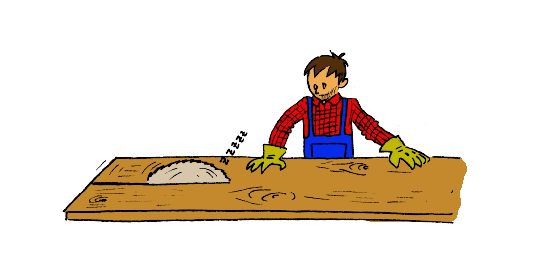
\includegraphics[width=5cm]{menuisier} \end{center}

Complète alors l'égalité $478,8 = 9 \times \ldots + \ldots$ . \label{NbEntDec_Approf81Qa}

 \item En utilisant la division écrite au \ref{NbEntDec_Approf81Qa}, recopie et complète les égalités suivantes :
 \begin{itemize}  
  \item $47,88 = 9 \times 5,3 + \ldots$ ;
  \item $4 788 = 9 \times 532 + \ldots$ ;
  \item $4 788 = 90 \times 53 + \ldots$ ;
  \item $4,788 = 9 \times \ldots + 0,018$.
  \end{itemize}
 \end{enumerate}
\end{exercice}


\begin{exercice}[Paquets empilés]
On a reçu au collège 7 rames de 500 feuilles pour la photocopieuse et 3 paquets de 24 pièces de « carton plume » :
\begin{enumerate}
 \item L'épaisseur d'une feuille de papier pour photocopieuse est de 0,11 mm et celle d'une pièce de « carton plume » est de 5 mm. Calcule un ordre de grandeur de la hauteur totale de tous ces paquets empilés ;
 \item Écris la hauteur totale des paquets en une seule expression puis calcule‑la.
 \end{enumerate}
\end{exercice}


\begin{exercice}[Densité de population]
On considère le tableau suivant :

\begin{center}
\begin{tabularx}{\linewidth}{|c|*{6}{>{\centering \arraybackslash}X|}}
\hline \rowcolor{U1} Continent & Nombre d'habitants & Superficie en km\up{2} \\
\hline \rowcolor{A3} Afrique & 965 millions & 30\,206\,704 \\
\hline \rowcolor{A3} Amérique & 911 millions & 42\,189\,120 \\
\hline \rowcolor{A3} Asie & 4,03 milliards & 43\,810\,582 \\
\hline \rowcolor{A3} Europe & 731 millions & 10\,180\,000 \\
\hline \rowcolor{A3} Océanie & 34 millions & 9\,008\,458 \\
\hline
\end{tabularx} \\
\end{center}

\begin{enumerate}
 \item Quel est le continent qui a le plus grand nombre d'habitants ? Et le plus petit nombre ?
 \item Quel est le continent qui a la plus grande superficie ? Et la plus petite ? 
 \end{enumerate}
\end{exercice}



